\documentclass[11pt]{exam}
\input{../../Header/packages.sty}
\input{../../Header/styleExam.sty}
\input{../../Header/headerQuestion.sty}
\input{../../Header/mathexpressions.sty}
%=========================================================
%\printanswers % einkommentieren, um statt der Antwortfelder die Lösungen anzuzeigen
\newcommand{\theme}{Wachstum \& Zerfall}
\newcommand{\teacher}{Jonas Guler}
\graphicspath{{data-algebra/}} % Setzt den Pfad zu den Bilder fest
%=========================================================
\begin{document}
\fontsize{14}{14}\selectfont
\begin{center}
    \huge\bf\theme
\end{center}

\begin{questions}
%=========================================================
%-------------------TESTFRAGEN
%=========================================================
\question[3]
Entschiede, ob die folgenden Funktionen eine Exponentialfunktion sind. Begründe deine Antwort.
\begin{parcols}[3]
    \part $y=3^{x-1}$
    \part $y=-3x+1$
    \part $y=\sqrt{3}^x+\frac{2}{3}$
    \part $y=0.2^{-x}$
    \part $y=2\*\left(\frac{1}{2^x}\right)$
    \part $y=x^3$
\end{parcols}
\ifthenelse{\boolean{printanswers}}
{\begin{solution}
		(a) Ja: $y=3^{x-1}=\frac{1}{3}\*3^x$ \quad (b) Nein: lineare Funktion, $x$ steht nicht im Exponenten.\\
		(c) Ja: Basis $\sqrt{3}$, der Graph ist um $\frac{2}{3}$ nach oben verschoben. \quad (d) Ja: $y=0.2^{-x}=5^x$\\
		(e) Ja: $y=2\*\left(\frac{1}{2}\right)^x$ \quad (f) Nein: Potenzfunktion, $x$ steht in der Basis.
\end{solution}}
{\antwort{6}}

%---------------------------------------------------------
\question[3]
Entschiede, ob die folgenden Funktionen eine Exponentialfunktion sind. Begründe deine Antwort.
\begin{parcols}[3]
    \part $y=3^{x-1}$
    \part $y=x^3$
    \part $y=0.2^{-x}$
    \part $y=2\*\left(\frac{1}{2}\right)^x-2$
    \part $y=-3x+1$
    \part $y=\sqrt{3}^x+\frac{2}{3}$
\end{parcols}
\ifthenelse{\boolean{printanswers}}
{\begin{solution}
		(a) Ja: $y=3^{x-1}=\frac{1}{3}\*3^x$ \quad (b) Nein: Potenzfunktion, $x$ steht in der Basis. \quad (c) Ja: $y=0.2^{-x}=5^x$\\
		(d) Ja: Basis $\frac{1}{2}$, der Graph ist um $2$ nach unten verschoben. \quad (e) Nein: lineare Funktion.\\
		(f) Ja: Basis $\sqrt{3}$, der Graph ist um $\frac{2}{3}$ nach oben verschoben.
\end{solution}}
{\antwort{6}}

%---------------------------------------------------------
\question[2]
Beschreibe in eigenen Worten, unter welcher Bedingung eine Funktion der Form $f(x)=b\*a^x$ wachsend bzw. fallend ist. Veranschauliche deine Aussage anhand zwei geeigneter Beispiele.
\ifthenelse{\boolean{printanswers}}
{\begin{solution}
		Für $b>0$ ist $f$ wachsend, wenn $a>1$, und fallend, wenn $0<a<1$ (für $b<0$ ist es umgekehrt).\\
		Beispiele: $f(x)=2\*3^x$ ist wachsend, $g(x)=5\*0.5^x$ ist fallend.
\end{solution}}
{\antwort{5}}

%---------------------------------------------------------
\question[2]
Skizziere die beiden Funktionen $f(x)=1.3^x$ und $g(x)=\left(\frac{1}{3}\right)^x$
\begin{figure}[H]
    \hspace{1cm}
    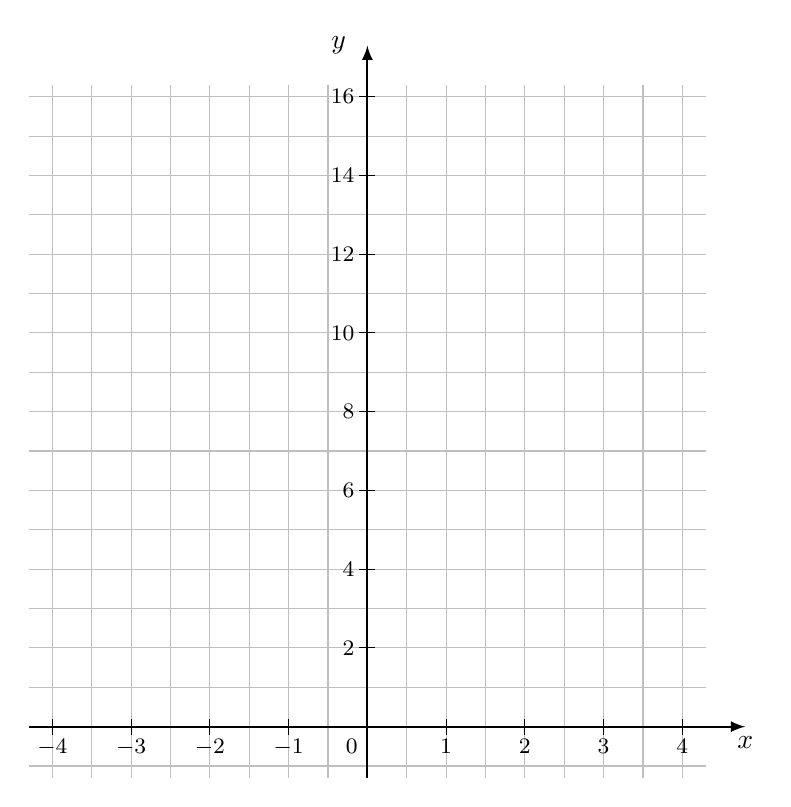
\begin{tikzpicture}[cross/.style={draw, cross out, minimum size=2*(#1-1pt), inner sep=0pt, outer sep=0pt}, x=10mm, y=5mm,
        >=latex,   %Voreinstellung für Pfeilspitzen
        font=\footnotesize, scale=1]
        %Raster zeichnen
        \draw [color=gray!50]  [step=5mm] (-4.3,-1.3) grid (4.3,16.3);
        % Achsen zeichnen
        \draw[->,thick] (-4.3,0) -- (4.8,0) node[left, below] {\normalsize $x$};
        \draw[->,thick] (0,-1.3) -- (0,17.3) node[above, left=4pt] {\normalsize $y$};
        % Achsen beschriften
        \foreach \x in {-4,-3,-2,-1,1,2,3,4} \draw (\x,-.2) -- (\x,.2) node[below=4pt] {$\x$};
        \foreach \y in {2,4,...,16} \draw (-.1,\y) -- (.1,\y) node[left=4pt] {$\y$};
        % Besserer Ursprung
        \draw[color=black] (0pt,-7pt) node[left] {$0$};
        %Funktionen zeichnen:
        \clip(-4.3,-1.3) rectangle (4.3,10.3); %Bildbereich
        %Beschriftung
        %\node[forestgreen]  at (3.2,1) {\normalsize$g$};
    \end{tikzpicture}
\end{figure}
\ifthenelse{\boolean{printanswers}}
{\begin{solution}
		Beide Graphen gehen durch $(0\,|\,1)$. $f$ wächst langsam ($f(-4)\approx0.35$, $f(4)\approx2.86$), $g$ fällt ($g(-2)=9$, $g(-1)=3$, $g(1)=\frac{1}{3}$).
		\begin{center}
		\begin{tikzpicture}[x=6mm, y=4mm, >=latex, font=\footnotesize]
			\draw[gray!50, step=1] (-4.3,-0.5) grid (4.3,10.3);
			\draw[->,thick] (-4.3,0) -- (4.8,0) node[below] {$x$};
			\draw[->,thick] (0,-0.5) -- (0,10.8) node[left] {$y$};
			\foreach \x in {-4,-2,2,4} \node[below] at (\x,0) {$\x$};
			\foreach \y in {2,4,...,10} \node[left] at (0,\y) {$\y$};
			\begin{scope}
				\clip (-4.3,-0.5) rectangle (4.3,10.3);
				\draw[plotblue, thick, domain=-4.3:4.3, samples=80] plot (\x,{1.3^\x}) node[above left] {$f$};
				\draw[forestgreen, thick, domain=-4.3:4.3, samples=80] plot (\x,{(1/3)^\x});
			\end{scope}
			\node[forestgreen] at (-2.6,9) {$g$};
		\end{tikzpicture}
		\end{center}
\end{solution}}
{\antwort{2.5}}

%---------------------------------------------------------
\question[2]
Skizziere die beiden Funktionen $f(x)=1.5^x$ und $g(x)=\left(\frac{2}{3}\right)^x$
\begin{figure}[H]
    \hspace{1cm}
    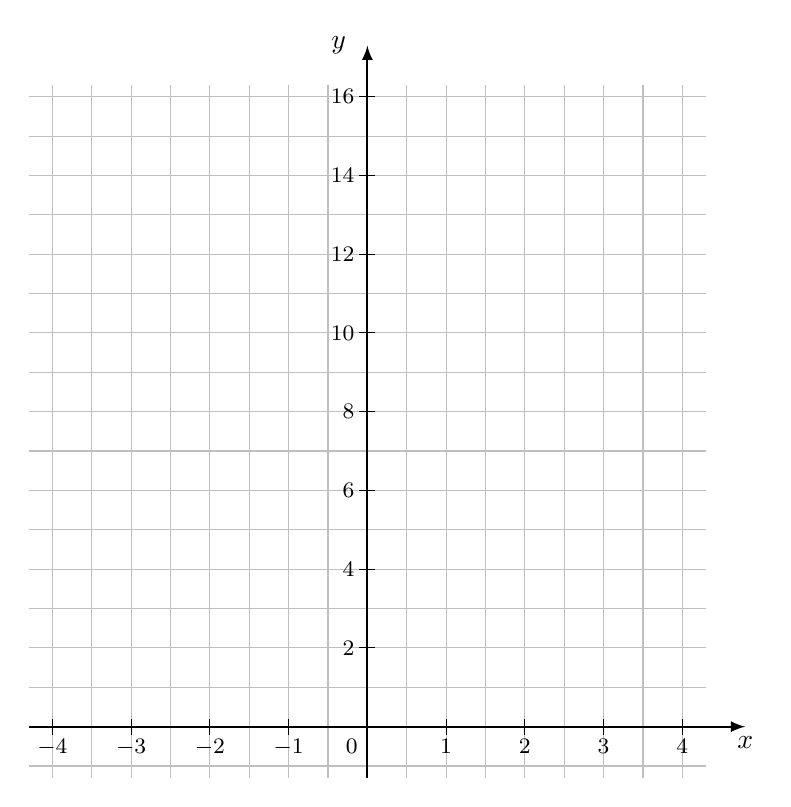
\begin{tikzpicture}[cross/.style={draw, cross out, minimum size=2*(#1-1pt), inner sep=0pt, outer sep=0pt}, x=10mm, y=5mm,
        >=latex,   %Voreinstellung für Pfeilspitzen
        font=\footnotesize, scale=1]
        %Raster zeichnen
        \draw [color=gray!50]  [step=5mm] (-4.3,-1.3) grid (4.3,16.3);
        % Achsen zeichnen
        \draw[->,thick] (-4.3,0) -- (4.8,0) node[left, below] {\normalsize $x$};
        \draw[->,thick] (0,-1.3) -- (0,17.3) node[above, left=4pt] {\normalsize $y$};
        % Achsen beschriften
        \foreach \x in {-4,-3,-2,-1,1,2,3,4} \draw (\x,-.2) -- (\x,.2) node[below=4pt] {$\x$};
        \foreach \y in {2,4,...,16} \draw (-.1,\y) -- (.1,\y) node[left=4pt] {$\y$};
        % Besserer Ursprung
        \draw[color=black] (0pt,-7pt) node[left] {$0$};
        %Funktionen zeichnen:
        \clip(-4.3,-1.3) rectangle (4.3,10.3); %Bildbereich
        %Beschriftung
        %\node[forestgreen]  at (3.2,1) {\normalsize$g$};
    \end{tikzpicture}
\end{figure}
\ifthenelse{\boolean{printanswers}}
{\begin{solution}
		Beide Graphen gehen durch $(0\,|\,1)$. Wegen $g(x)=\left(\frac{2}{3}\right)^x=1.5^{-x}=f(-x)$ ist $g$ das Spiegelbild von $f$ an der $y$-Achse ($f(2)=2.25$, $f(4)\approx5.06$).
		\begin{center}
		\begin{tikzpicture}[x=6mm, y=4mm, >=latex, font=\footnotesize]
			\draw[gray!50, step=1] (-4.3,-0.5) grid (4.3,10.3);
			\draw[->,thick] (-4.3,0) -- (4.8,0) node[below] {$x$};
			\draw[->,thick] (0,-0.5) -- (0,10.8) node[left] {$y$};
			\foreach \x in {-4,-2,2,4} \node[below] at (\x,0) {$\x$};
			\foreach \y in {2,4,...,10} \node[left] at (0,\y) {$\y$};
			\begin{scope}
				\clip (-4.3,-0.5) rectangle (4.3,10.3);
				\draw[plotblue, thick, domain=-4.3:4.3, samples=80] plot (\x,{1.5^\x}) node[above left] {$f$};
				\draw[forestgreen, thick, domain=-4.3:4.3, samples=80] plot (\x,{(2/3)^\x});
			\end{scope}
			\node[forestgreen] at (-3.6,9) {$g$};
		\end{tikzpicture}
		\end{center}
\end{solution}}
{\antwort{2.5}}

%---------------------------------------------------------
\question[3]
Im folgenden sind drei Wertetabellen gegeben. Entscheide für jede Wertetabelle, ob es sich um eine Exponentialfunktion handelt. Wenn ja, gib die Funktionsgleichung an.
\begin{parcols}[3]
    \part \
        \begin{table}[H]
            \begin{tabular}{|c|c|c|c|c|}\hline
                $x$ & 1 & 2 & 3 & 4 \\\hline
                $f(x)$ & 4 & 16 & 64 & 256 \\\hline
            \end{tabular}
        \end{table}
    \part \
        \begin{table}[H]
            \begin{tabular}{|c|c|c|c|c|}\hline
                $x$ & 1 & 2 & 3 & 4 \\\hline
                $f(x)$ & -6 & 2 & 10 & 18 \\\hline
            \end{tabular}
        \end{table}
    \part\
        \begin{table}[H]
            \begin{tabular}{|c|c|c|c|c|}\hline
                $x$ & 1 & 2 & 3 & 4 \\\hline
                $f(x)$ & 20 & 5 & $\frac{5}{4}$ & $\frac{5}{16}$ \\\hline
            \end{tabular}
        \end{table}
\end{parcols}
\ifthenelse{\boolean{printanswers}}
{\begin{solution}
		(a) Exponentiell, konstanter Faktor $4$: $f(x)=4^x$.\\
		(b) Nicht exponentiell: konstante Differenz $8$, also linear ($f(x)=8x-14$).\\
		(c) Exponentiell, konstanter Faktor $\frac{1}{4}$: $f(x)=80\*\left(\frac{1}{4}\right)^x$.
\end{solution}}
{\antwort{6}}


%---------------------------------------------------------
\question[3]
Im folgenden sind drei Wertetabellen gegeben. Entscheide für jede Wertetabelle, ob es sich um eine Exponentialfunktion handelt. Wenn ja, gib die Funktionsgleichung an.
\begin{parcols}[3]
	\part \
	\begin{table}[H]
		\begin{tabular}{|c|c|c|c|c|}\hline
			$x$ & 1 & 2 & 3 & 4 \\\hline
			$f(x)$ & 3 & 9 & 27 & 81 \\\hline
		\end{tabular}
	\end{table}
	\part \
	\begin{table}[H]
		\begin{tabular}{|c|c|c|c|c|}\hline
			$x$ & 1 & 2 & 3 & 4 \\\hline
			$f(x)$ & -7 & -2 & 3 & 8 \\\hline
		\end{tabular}
	\end{table}
	\part\
	\begin{table}[H]
		\begin{tabular}{|c|c|c|c|c|}\hline
			$x$ & 1 & 2 & 3 & 4 \\\hline
			$f(x)$ & 32 & 8 & 2 & $\frac{2}{4}$ \\\hline
		\end{tabular}
	\end{table}
\end{parcols}
\ifthenelse{\boolean{printanswers}}
{\begin{solution}
		(a) Exponentiell, konstanter Faktor $3$: $f(x)=3^x$.\\
		(b) Nicht exponentiell: konstante Differenz $5$, also linear ($f(x)=5x-12$).\\
		(c) Exponentiell, konstanter Faktor $\frac{1}{4}$: $f(x)=128\*\left(\frac{1}{4}\right)^x$.
\end{solution}}
{\antwort{6}}


%---------------------------------------------------------
\noaddpoints
\question[\totalpoints]
\addpoints
Beantworte für die beiden Funktionen $f:y=a\*x$ und $g:y=a^x$ die folgenden Fragen: Wie verändert sich der Funktionswert, ...
\begin{parts}
    \part[2] ... wenn man den $x-$Wert um 6 erhöht?
    \part[2] ... wenn man den $x-$Wert um 4 verkleinert?
\end{parts}
\ifthenelse{\boolean{printanswers}}
{\begin{solution}
		(a) $f(x+6)=a\*x+6a$: Der Funktionswert von $f$ wird um $6a$ grösser. $g(x+6)=a^x\*a^6$: Der Funktionswert von $g$ wird mit $a^6$ multipliziert.\\
		(b) $f(x-4)=a\*x-4a$: Der Funktionswert von $f$ wird um $4a$ kleiner. $g(x-4)=\frac{a^x}{a^4}$: Der Funktionswert von $g$ wird durch $a^4$ dividiert.
\end{solution}}
{\antwort{8.5}}


%---------------------------------------------------------
\noaddpoints
\question[\totalpoints]
\addpoints
Beantworte für die beiden Funktionen $f:y=a\*x$ und $g:y=a^x$ die folgenden Fragen: Wie verändert sich der Funktionswert, ...
\begin{parts}
    \part[2] ... wenn man den $x-$Wert um 4 erhöht?
    \part[2] ... wenn man den $x-$Wert halbiert?
\end{parts}
\ifthenelse{\boolean{printanswers}}
{\begin{solution}
		(a) $f(x+4)=a\*x+4a$: Der Funktionswert von $f$ wird um $4a$ grösser. $g(x+4)=a^x\*a^4$: Der Funktionswert von $g$ wird mit $a^4$ multipliziert.\\
		(b) $f(\frac{x}{2})=\frac{1}{2}\*a\*x$: Der Funktionswert von $f$ wird halbiert. $g(\frac{x}{2})=a^{\frac{x}{2}}=\sqrt{a^x}$: Aus dem Funktionswert von $g$ wird die Quadratwurzel gezogen.
\end{solution}}
{\antwort{8.5}}


%---------------------------------------------------------
\noaddpoints
\question[\totalpoints]
\addpoints
Beantworte für die beiden Funktionen $f:y=a\*x$ und $g:y=a^x$ die folgenden Fragen: Wie verändert sich der Funktionswert, ...
\begin{parts}
	\part[2] ... wenn man den $x-$Wert um 4 verringert?
	\part[2] ... wenn man den $x-$Wert verdreifacht?
\end{parts}
\ifthenelse{\boolean{printanswers}}
{\begin{solution}
		(a) $f(x-4)=a\*x-4a$: Der Funktionswert von $f$ wird um $4a$ kleiner. $g(x-4)=\frac{a^x}{a^4}$: Der Funktionswert von $g$ wird durch $a^4$ dividiert.\\
		(b) $f(3x)=3\*a\*x$: Der Funktionswert von $f$ wird verdreifacht. $g(3x)=a^{3x}=\left(a^x\right)^3$: Der Funktionswert von $g$ wird hoch $3$ genommen.
\end{solution}}
{\antwort{8.5}}

%---------------------------------------------------------
\noaddpoints
\question[\totalpoints]
\addpoints
Betrachte die beiden Funktionen $f:y=a\*x$ und $g:y=a^x$. Wie lautet die Funktionsgleichung, wenn bei jeder Erhöhung von $x$ um $1$ ...
\begin{parts}
    \part[2] ... der Funktionswert verdreifacht wird?
    \part[2] ... der Funktionswert um $20\%$ zunimmt?
\end{parts}
\ifthenelse{\boolean{printanswers}}
{\begin{solution}
		Bei $f$ wird pro Schritt immer derselbe Betrag $a$ addiert, das Verhältnis $\frac{f(x+1)}{f(x)}=\frac{x+1}{x}$ hängt von $x$ ab. Für $f$ gibt es deshalb in (a) und (b) keine passende Gleichung. Bei $g$ wird pro Schritt mit $a$ multipliziert:\\
		(a) $g:y=3^x$ \qquad (b) $g:y=1.2^x$
\end{solution}}
{\antwort{8.5}}


%---------------------------------------------------------
\question[6]
Ordne die Graphen den Funktionsgleichungen zu. Begründe deine Antwort.\\
\begin{minipage}{0.45\linewidth}
    \centering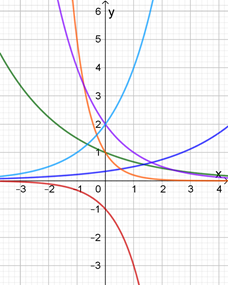
\includegraphics[scale=3]{expGraph.png}
\end{minipage}
\hfill
\begin{minipage}{0.45\linewidth}
    \begin{parts}
    \part $f_1(x)=2\cdot0.5^x$
    \part $f_2(x)=-3^x$
    \part $f_3(x)=\left(\frac{2}{3}\right)^x$
    \part $f_4(x)=\frac{1}{3}\cdot1.5^x$
    \part $f_5(x)=0.2^x$
    \part $f_6(x)=2\cdot 2^x$
\end{parts}
\end{minipage}
\ifthenelse{\boolean{printanswers}}
{\begin{solution}
		Zuordnung über den $y$-Achsenabschnitt $b$ und die Basis $a$:\\
		(a) $f_1$: fallend durch $(0\,|\,2)$ (violett). \quad (b) $f_2$: negativ, durch $(0\,|\,-1)$ (rot).\\
		(c) $f_3$: langsam fallend durch $(0\,|\,1)$ (dunkelgrün). \quad (d) $f_4$: langsam steigend durch $(0\,|\,\frac{1}{3})$ (dunkelblau).\\
		(e) $f_5$: schnell fallend durch $(0\,|\,1)$ (orange). \quad (f) $f_6$: steigend durch $(0\,|\,2)$ (hellblau).
\end{solution}}
{\antwort{6}}

%---------------------------------------------------------
\question[4]
Am Eröffnungstag eines Streichelzoos befanden sich $93$ Meerschweinchen in einem Gehege. Ein Jahr später waren es bereits $115$.
\begin{parts}
    \part Wie viele Meerschweinchen werden es am Tag des $10-$jährigen Jubiläums sein, wenn wir ein lineares Wachstum annehmen?
    \part Wie viele Meerschweinchen werden es am Jubiläumstag sein, wenn wir ein exponentielles Wachstum annehmen?
\end{parts}
\ifthenelse{\boolean{printanswers}}
{\begin{solution}
		(a) Zunahme $22$ pro Jahr: $N(10)=93+10\*22=313$ Meerschweinchen.\\
		(b) Faktor $\frac{115}{93}\approx1.2366$ pro Jahr: $N(10)=93\*\left(\frac{115}{93}\right)^{10}\approx777$ Meerschweinchen.
\end{solution}}
{\antwort{8}}

%---------------------------------------------------------
\question[4]
Als eine Gemeinde ihr Förderprogramm für Solaranlagen startete, waren auf ihren Hausdächern $250$ Solaranlagen installiert. Ein Jahr später waren es bereits $310$.
\begin{parts}
	\part Wie viele Solaranlagen werden es am Tag des $10-$jährigen Jubiläums des Förderprogramms sein, wenn wir ein lineares Wachstum annehmen?
	\part Wie viele Solaranlagen werden es am Jubiläumstag sein, wenn wir ein exponentielles Wachstum annehmen?
\end{parts}
\ifthenelse{\boolean{printanswers}}
{\begin{solution}
		(a) Zunahme $60$ pro Jahr: $N(10)=250+10\*60=850$ Solaranlagen.\\
		(b) Faktor $\frac{310}{250}=1.24$ pro Jahr: $N(10)=250\*1.24^{10}\approx2'149$ Solaranlagen.
\end{solution}}
{\antwort{8}}


%---------------------------------------------------------
\question[4]
In einem See verringert sich die Intensität des Lichtes mit jedem Meter Wassertiefe um $40\%$.
\begin{parts}
    \part Stelle ein Zerfallsgesetz auf, das die Wassertiefe in Meter der Lichtintensität in Prozent zuordnet.
    \part In welcher Wassertiefe beträgt die Lichtintensität noch $5\%$ der Intensität über der Wasseroberfläche?
\end{parts}
\ifthenelse{\boolean{printanswers}}
{\begin{solution}
		(a) $I(h)=100\*0.6^h$ ($h$ in Metern, $I$ in Prozent).\\
		(b) $100\*0.6^h=5\ \Rightarrow\ h=\frac{\ln{0.05}}{\ln{0.6}}\approx5.86$ m.
\end{solution}}
{\antwort{8}}

%---------------------------------------------------------
\question[4] %DMK 9-10 A25
Ein Kapital von $1000.-$ CHF wird bei einer Bank angelegt. Der Zins wird jeweils am Ende der Zinsperiode zu Kapital addiert. Berechne das Kapital nach 10 Jahren, wenn...
\begin{parts}
    \part ... das Kapital jährlich zu $1\%$ verzinst wird.
    \part ... das Kapital monatlich zu $\frac{1}{12}\%$ verzinst wird.
\end{parts}
Welche Variante würdest du bevorzugen? Begründe.
\ifthenelse{\boolean{printanswers}}
{\begin{solution}
		(a) $K_{10}=1000\*1.01^{10}\approx1'104.62$ CHF \qquad (b) $K_{10}=1000\*\left(1+\frac{0.01}{12}\right)^{120}\approx1'105.12$ CHF\\
		Die monatliche Verzinsung ist (knapp $50$ Rappen) besser, weil die Zinsen früher mitverzinst werden (Zinseszins).
\end{solution}}
{\antwort{8}}

%---------------------------------------------------------
\question[5]
Von einem neu entdeckten radioaktiven Element namens Heerbruggium zerfallen in $7$ Minuten $10\%$ seines noch vorhandenen Bestandes.
\begin{parts}
    \part Berechne seine Halbwertszeit.
    \part Wie viel Prozent seines noch vorhandenen Bestandes zerfallen in der nächsten Stunde?
\end{parts}
\ifthenelse{\boolean{printanswers}}
{\begin{solution}
		Faktor pro $7$ Minuten: $0.9$, also $N(t)=N_0\*0.9^{\frac{t}{7}}$ ($t$ in Minuten).\\
		(a) $0.9^{\frac{T}{7}}=0.5\ \Rightarrow\ T=7\*\frac{\ln{0.5}}{\ln{0.9}}\approx46.05$ Minuten.\\
		(b) $0.9^{\frac{60}{7}}\approx0.4053$. In der nächsten Stunde zerfallen rund $59.5\%$ des Bestandes.
\end{solution}}
{\antwort{10}}

%---------------------------------------------------------
\question[5]
Ein neu entwickeltes Schmerzmittel namens Analgetin wird vom Körper so abgebaut, dass in $5$ Stunden jeweils $20\%$ der noch im Blut vorhandenen Wirkstoffmenge abgebaut werden.
\begin{parts}
	\part Berechne die Halbwertszeit des Wirkstoffs im Blut.
	\part Wie viel Prozent der noch vorhandenen Wirkstoffmenge werden im Lauf des nächsten Tages ($24$ Stunden) abgebaut?
\end{parts}
\ifthenelse{\boolean{printanswers}}
{\begin{solution}
		Faktor pro $5$ Stunden: $0.8$, also $M(t)=M_0\*0.8^{\frac{t}{5}}$ ($t$ in Stunden).\\
		(a) $0.8^{\frac{T}{5}}=0.5\ \Rightarrow\ T=5\*\frac{\ln{0.5}}{\ln{0.8}}\approx15.53$ Stunden.\\
		(b) $0.8^{\frac{24}{5}}\approx0.3426$. Im Lauf eines Tages werden rund $65.7\%$ des Wirkstoffs abgebaut.
\end{solution}}
{\antwort{10}}

%---------------------------------------------------------
\question[6]
Die Vermehrung von Keimen in Kuhmilch lässt sich durch eine Exponentialfunktion beschreiben. In $1$ cm$^3$ Kuhmilch werden $3$ Stunden nach dem Melken $66'000$ Keime nachgewiesen. $2$ Stunden später sind es bereits $1.1$ Millionen Keime.
\begin{parts}
    \part Berechne die Anzahl der Keime $6$ Stunden nach dem Melken.
    \part In welcher Zeit verdreifacht sich die Anzahl der Keime?
    \part Um wie viele Prozent wächst die Anzahl der Keime innerhalb einer Stunde?
\end{parts}
\ifthenelse{\boolean{printanswers}}
{\begin{solution}
		Ansatz $N(t)=b\*a^t$ ($t$ in Stunden): $a^2=\frac{1'100'000}{66'000}=\frac{50}{3}\Rightarrow a\approx4.0825$ und $b=\frac{66'000}{a^3}\approx970$.\\
		(a) $N(6)=1'100'000\*a\approx4.49$ Millionen Keime.\\
		(b) $a^t=3\Rightarrow t=\frac{\ln{3}}{\ln{a}}\approx0.78$ Stunden (etwa $47$ Minuten).\\
		(c) $a\approx4.08$: Die Anzahl der Keime wächst pro Stunde um rund $308\%$.
\end{solution}}
{\antwort{12}}

%---------------------------------------------------------
\question[6]
Die Verbreitung eines viralen Videos auf einer Online-Plattform lässt sich in der Anfangsphase durch eine Exponentialfunktion beschreiben. $2$ Tage nach dem Hochladen wurde das Video $40'000$-mal aufgerufen. $2$ Tage später sind es bereits $900'000$ Aufrufe.
\begin{parts}
	\part Berechne die Anzahl der Aufrufe $5$ Tage nach dem Hochladen.
	\part In welcher Zeit verdreifacht sich die Anzahl der Aufrufe?
	\part Um wie viele Prozent wächst die Anzahl der Aufrufe innerhalb eines Tages?
\end{parts}
\ifthenelse{\boolean{printanswers}}
{\begin{solution}
		Ansatz $N(t)=b\*a^t$ ($t$ in Tagen): $a^2=\frac{900'000}{40'000}=22.5\Rightarrow a\approx4.7434$ und $b=\frac{40'000}{22.5}\approx1'778$.\\
		(a) $N(5)=900'000\*a\approx4.27$ Millionen Aufrufe.\\
		(b) $a^t=3\Rightarrow t=\frac{\ln{3}}{\ln{a}}\approx0.71$ Tage (etwa $17$ Stunden).\\
		(c) $a\approx4.74$: Die Anzahl der Aufrufe wächst pro Tag um rund $374\%$.
\end{solution}}
{\antwort{12}}

%---------------------------------------------------------
\question[4] %Ss
Eine Pilzkultur an einer Kellerwand wird in einem Beobachtungszeitraum von drei Monaten chemisch so behandelt, dass ihre Fläche jede Woche um $11\%$ abnimmt. Zu Beginn des Zeitraums bedeckt sie eine Fläche von $2.4\:m^2$.
\begin{parts}
    \part Welche Fläche bedeckt sie am Ende des Beobachtungszeitraums?
    \part Wie viele Tage muss die Behandlung insgesamt dauern, dass die Pilzkultur höchstens noch eine Fläche von $0.1\:m^2$ bedeckt?
\end{parts}
\ifthenelse{\boolean{printanswers}}
{\begin{solution}
		$A(w)=2.4\*0.89^w$ ($w$ in Wochen, $A$ in m$^2$).\\
		(a) Drei Monate sind etwa $13$ Wochen: $A(13)=2.4\*0.89^{13}\approx0.53$ m$^2$.\\
		(b) $2.4\*0.89^w=0.1\ \Rightarrow\ w=\frac{\ln{\frac{0.1}{2.4}}}{\ln{0.89}}\approx27.27$ Wochen, also rund $191$ Tage.
\end{solution}}
{\antwort{8}}

%---------------------------------------------------------
\question[6]
Die Entwicklung der wöchentlichen Corona-Fallzahlen verlief in gewissen Zeiträumen annähernd exponentiell. Im Jahr $2021$ wurden in der Kalenderwoche $44$ insgesamt $17'203$ und in der Kalenderwoche $45$ insgesamt $24'823$ positive Fälle gemeldet. Unter der Annahme eines exponentiellen Wachstums der positiven Fälle berechne das Folgende:
\begin{parts}
    \part Bestimme die prozentuale wöchentliche Zunahme.
    \part Wie viele Fälle sind in der Kalenderwoche $48$ zu erwarten?
    \part In welchem Zeitraum (in Tagen) verdoppeln sich die positiven Fälle?
    \part Wir nehmen an, das exponentielle Wachstum setzt sich ungebremst fort. In welcher Kalenderwoche wäre erstmals mit mehr als $250'000$ Fälle pro Woche zu rechnen?
\end{parts}
\ifthenelse{\boolean{printanswers}}
{\begin{solution}
		(a) $a=\frac{24'823}{17'203}\approx1.4429$: wöchentliche Zunahme rund $44.3\%$.\\
		(b) $N_{48}=24'823\*a^3\approx74'577$ Fälle.\\
		(c) $a^t=2\Rightarrow t=\frac{\ln{2}}{\ln{a}}\approx1.89$ Wochen, also rund $13.2$ Tage.\\
		(d) $24'823\*a^n>250'000\Rightarrow n>\frac{\ln{\frac{250'000}{24'823}}}{\ln{a}}\approx6.30$ Wochen nach KW $45$, also erstmals in KW $52$.
\end{solution}}
{\antwort{14}}

%---------------------------------------------------------
\question[4] %Ss
Faltet man ein Stück Papier im DIN Format mehrfach längs der Mittellinie, so liegen erst zwei, dann vier Schichten,... übereinander. Es wird dabei immer kleiner und dicker. Wie oft müsste das Blatt gefaltet werden, um einen Turm, der bis zum Mond reicht, zu erhalten?\\
(Entfernung zum Mond: $384'000\:km$, Papierdicke: $0.1\:mm$)
\ifthenelse{\boolean{printanswers}}
{\begin{solution}
		Nach $n$ Faltungen ist der Stapel $0.1\*2^n$ mm dick. Mit $384'000$ km $=3.84\*10^{11}$ mm:\\
		$0.1\*2^n\geq3.84\*10^{11}\ \Rightarrow\ 2^n\geq3.84\*10^{12}\ \Rightarrow\ n\geq\frac{\ln{3.84\*10^{12}}}{\ln{2}}\approx41.8$\\
		Das Blatt müsste $42$-mal gefaltet werden.
\end{solution}}
{\antwort{8}}

%---------------------------------------------------------
\question[4] %DMK 9-10 A25
Ein Kapital von $1000.-$ CHF wird bei einer Bank angelegt. Der Zins wird jeweils am Ende der Zinsperiode zu Kapital addiert. Berechne das Kapital nach 10 Jahren, wenn
\begin{itemize}
    \item das Kapital jährlich zu $1\%$ verzinst wird.
    \item das Kapital monatlich zu $\frac{1}{12}\%$ verzinst wird.
\end{itemize}
Vergleiche nun die beiden Zinsvarianten. Welche Variante würdest du bevorzugen? Begründe.
\ifthenelse{\boolean{printanswers}}
{\begin{solution}
		Jährlich: $K_{10}=1000\*1.01^{10}\approx1'104.62$ CHF. \quad Monatlich: $K_{10}=1000\*\left(1+\frac{0.01}{12}\right)^{120}\approx1'105.12$ CHF.\\
		Die monatliche Verzinsung ist (knapp $50$ Rappen) besser, weil die Zinsen früher mitverzinst werden (Zinseszins).
\end{solution}}
{\antwort{8}}

%---------------------------------------------------------
\question[6]
Vor $10$ Jahren betrug der Holzbestand eines Waldes $7'000$ m$^3$. Ohne Abholzen ist er inzwischen auf $9'880$ m$^3$ angewachsen. Man darf annehmen, dass daas Holzwachstum ein exponentieller Vorgang ist.
\begin{parts}
    \part Bestimme die jährliche Wachstumsrate.
    \part Berechne die Zeitspanne, innerhalb der sich der Holzbestand verdoppelt.
    \part Der Besitzer plant, in $3$ Jahren $3'000$ m$^3$ Holz zu schlagen. Wann wird dieser Wald den heutigen Holzbestand wieder erreichen.
\end{parts}
\ifthenelse{\boolean{printanswers}}
{\begin{solution}
		(a) $a^{10}=\frac{9'880}{7'000}\Rightarrow a=\sqrt[10]{\frac{9'880}{7'000}}\approx1.0351$: jährliche Wachstumsrate rund $3.5\%$.\\
		(b) $a^t=2\Rightarrow t=\frac{\ln{2}}{\ln{a}}\approx20.1$ Jahre.\\
		(c) In $3$ Jahren: $9'880\*a^3\approx10'956$ m$^3$, nach dem Schlagen bleiben $7'956$ m$^3$.\\
		$7'956\*a^t=9'880\Rightarrow t=\frac{\ln{\frac{9'880}{7'956}}}{\ln{a}}\approx6.3$ Jahre nach dem Schlagen, also in rund $9.3$ Jahren ab heute.
\end{solution}}
{\antwort{12}}

%---------------------------------------------------------
\noaddpoints
\question[\totalpoints] %NeueWege
\addpoints
Im Jahr $1950$ lebten $2.5$ Milliarden Menschen auf der Erde, $1980$ waren es dann $4.5$ Milliarden.
\begin{parts}
    \part[2] Stelle eine Wachstumsfunktion auf, die das Bevölkerungswachstum oben beschreibt.
    \part[2] Bestimme die Verdoppelungszeit
    \part[2] Vergleiche dein Resultat mit den Daten von $2005$ ($6.4$ Milliarden) und $1920$ ($1.8$ Milliarden). Was fällt dir auf?
    \part[2] $2005$ prognostizierten Experten der Vereinten Nationen bis zum Jahr $2050$
    einen Anstieg auf $9.1$ Milliarden. Wie lautet deine Prognose?
\end{parts}
\ifthenelse{\boolean{printanswers}}
{\begin{solution}
		(a) $N(t)=2.5\*a^t$ ($t$ in Jahren ab $1950$, $N$ in Milliarden) mit $a=\sqrt[30]{1.8}\approx1.0198$.\\
		(b) $a^t=2\Rightarrow t=\frac{\ln{2}}{\ln{a}}\approx35.4$ Jahre.\\
		(c) Modell: $N(55)\approx7.3$ Mrd. für $2005$ (statt $6.4$) und $N(-30)=\frac{2.5}{1.8}\approx1.4$ Mrd. für $1920$ (statt $1.8$). Das Wachstum war vor $1950$ langsamer und ist nach $1980$ wieder langsamer geworden, es ist also nicht über die ganze Zeit exponentiell.\\
		(d) Modell: $N(100)=2.5\*1.8^{\frac{10}{3}}\approx17.7$ Mrd. Da sich das Wachstum abschwächt, ist eine Prognose deutlich darunter (z.\,B. die $9.1$ Mrd. der UNO) realistischer.
\end{solution}}
{\antwort{14}}

%---------------------------------------------------------
\question[6]
Im Jahr $1945$ lebten $4.2$ Millionen Menschen in der Schweiz, $1967$ waren es dann $6.9$ Millionen.
\begin{parts}
    \part Stelle eine Wachstumsfunktion auf, die den Prozess oben beschreibt.
    \part Bestimme die Verdoppelungszeit.
    \part Vergleiche das Wachstum aus (a) mit den neuen erhobenen Daten von $2005$ ($7.3$ Millionen) und $1900$ ($3.4$ Millionen). Beschreibe in eigenen Worten, was dir dabei auffällt.
\end{parts}
\ifthenelse{\boolean{printanswers}}
{\begin{solution}
		(a) $N(t)=4.2\*a^t$ ($t$ in Jahren ab $1945$, $N$ in Millionen) mit $a=\sqrt[22]{\frac{6.9}{4.2}}\approx1.0228$.\\
		(b) $a^t=2\Rightarrow t=\frac{\ln{2}}{\ln{a}}\approx30.7$ Jahre.\\
		(c) Modell: $N(60)\approx16.3$ Mio. für $2005$ (statt $7.3$) und $N(-45)\approx1.5$ Mio. für $1900$ (statt $3.4$). Das starke Wachstum der Nachkriegszeit war eine Ausnahme, über längere Zeit wächst die Bevölkerung viel langsamer als exponentiell mit $2.3\%$.
\end{solution}}
{\antwort{12}}

%---------------------------------------------------------
\question[8]
\begin{parts}
    \part Im Jahr $1945$ lebten $4.2$ Millionen Menschen in der Schweiz, $1967$ waren es dann $6.9$ Millionen. Modelliere das Bevölkerungswachstum und bestimme die Verdoppelungszeit.
    \part Vergleiche das Wachstum aus (a) mit den neuen Daten von $2005$ ($7.3$ Millionen) und $1900$ ($3.4$ Millionen). Was fällt dir auf?
    \part $2005$ prognostizierten Experten des Bundesamtes für Statistik bis zum Jahr $2050$ einen Anstieg auf $9.5$ Millionen. Wie lautet deine Prognose?
\end{parts}
\ifthenelse{\boolean{printanswers}}
{\begin{solution}
		(a) $N(t)=4.2\*a^t$ ($t$ in Jahren ab $1945$, $N$ in Millionen) mit $a=\sqrt[22]{\frac{6.9}{4.2}}\approx1.0228$. Verdoppelungszeit: $t=\frac{\ln{2}}{\ln{a}}\approx30.7$ Jahre.\\
		(b) Modell: $N(60)\approx16.3$ Mio. für $2005$ (statt $7.3$) und $N(-45)\approx1.5$ Mio. für $1900$ (statt $3.4$). Das starke Wachstum der Nachkriegszeit war eine Ausnahme, über längere Zeit wächst die Bevölkerung viel langsamer.\\
		(c) Modell: $N(105)\approx44.9$ Mio. für $2050$. Das ist unrealistisch, eine Prognose in der Grössenordnung von $9.5$ Mio. (Bundesamt für Statistik) ist plausibler.
\end{solution}}
{\antwort{14}}

%---------------------------------------------------------
\noaddpoints
\question[\totalpoints]
\addpoints
Eine Computeranlage mit Neuwert $2056900.-$ CHF wird nach $6.5$ Jahren für $400000.-$ CHF verkauft.
\begin{parts}
    \part[2] Wie viel Prozent beträgt die mittlere jährliche Wertabnahme?
    \part[3] Nach $20$ Jahren möchten neue Investoren die Anlage wieder auf den neusten Stand bringen. Wie viel Geld müssten investiert werden, um wieder auf den Neuwert zu gelangen?
\end{parts}
\ifthenelse{\boolean{printanswers}}
{\begin{solution}
		(a) $a^{6.5}=\frac{400'000}{2'056'900}\Rightarrow a=\sqrt[6.5]{\frac{400'000}{2'056'900}}\approx0.7773$: mittlere jährliche Wertabnahme rund $22.3\%$.\\
		(b) Wert nach $20$ Jahren: $2'056'900\*a^{20}\approx13'337$ CHF. Investiert werden müssten $2'056'900-13'337\approx2'043'563$ CHF.
\end{solution}}
{\antwort{10}}

%---------------------------------------------------------
\question[2]
Entscheide in der Tabelle unten, ob die Aussagen wahr oder falsch sind. Die Antworten müssen nicht begründet werden.\newline
\begin{small}
    Bewertung: Für $0-2$ korrekte Antworten gibt es keine Punkte; $3$ korrekte Antworten einen Punkt und falls alle Antworten korrekt sind, gibt es $2$ Punkte.
\end{small}
\begingroup
\renewcommand{\arraystretch}{1.5}
\begin{table}[h]
    \centering
    \begin{tabular}{|p{12cm}|c|c|}\hline
         & wahr & falsch \\\hline
        Wenn eine Grösse jährlich um $7\%$ wächst, dann wächst sie in zwei Jahren um exakt 14\%. & & \\\hline
        Eine Funktion $f(t)=200\*0.65^t$ beschreibt einen exponentiellen Prozess, bei dem eine Grösse pro Zeiteinheit um $35\%$ abnimmt. & & \\\hline
        Eine Funktion $f(t)=200\*1.7^t$ beschreibt einen exponentiellen Prozess, bei dem eine Grösse pro Zeiteinheit um $170\%$ zunimmt. & & \\\hline
        Eine Funktion $f(t)=200\*\left(\frac{1}{\sqrt{2}}\right)^t$ beschreibt einen exponentiellen Prozess, bei dem sich eine Grösse alle zwei Jahre halbiert. & & \\\hline
        Eine Funktion $f(t)=200\*0.75^t$ beschreibt einen exponentiellen Prozess, bei dem eine Grösse pro Zeiteinheit um $25\%$ abnimmt. & & \\\hline
        Eine Funktion $f(t)=200\*\left(\frac{1}{\sqrt{2}}\right)^t$ beschreibt einen exponentiellen Prozess, bei dem sich eine Grösse alle zwei Jahre halbiert. & & \\\hline
        Wenn eine Grösse jährlich um $9\%$ wächst, dann wächst sie in zwei Jahren um exakt $18\%$. & & \\\hline
        Eine Funktion $f(t)=200\*1.7^t$ beschreibt einen exponentiellen Prozess, bei dem eine Grösse pro Zeiteinheit um $170\%$ zunimmt. & & \\\hline
        Wenn eine Grösse jährlich um $7\%$ wächst, dann wächst sie in zwei Jahren um exakt 14\%. & & \\\hline
        Eine Funktion $f(t)=200\*0.65^t$ beschreibt einen exponentiellen Prozess, bei dem eine Grösse pro Zeiteinheit um $35\%$ abnimmt. & & \\\hline
        Eine Funktion $f(t)=200\*1.7^t$ beschreibt einen exponentiellen Prozess, bei dem eine Grösse pro Zeiteinheit um $170\%$ zunimmt. & & \\\hline
        Eine Funktion $f(t)=200\*\left(\frac{1}{\sqrt{2}}\right)^t$ beschreibt einen exponentiellen Prozess, bei dem sich eine Grösse alle zwei Jahre halbiert. & & \\\hline
        Eine Funktion $f(t)=200\*0.55^t$ beschreibt einen exponentiellen Prozess, bei dem eine Grösse pro Zeiteinheit um $55\%$ abnimmt. & & \\\hline
        Eine Funktion $f(t)=200\*\left(\frac{1}{\sqrt{2}}\right)^t$ beschreibt einen exponentiellen Prozess, bei dem sich eine Grösse alle zwei Jahre halbiert. & & \\\hline
        Wenn eine Grösse jährlich um $10\%$ abnimmt, dann nimmt sie in zwei Jahren um exakt $19\%$ ab. & & \\\hline
        Eine Funktion $f(t)=200\*1.3^t$ beschreibt einen exponentiellen Prozess, bei dem eine Grösse pro Zeiteinheit um $30\%$ zunimmt. & & \\\hline
    \end{tabular}
\end{table}
\endgroup
\ifthenelse{\boolean{printanswers}}
{\begin{solution}
		Von oben nach unten:\\
		1.~falsch ($1.07^2=1.1449$, also $14.49\%$) \quad 2.~wahr \quad 3.~falsch (Zunahme $70\%$) \quad 4.~wahr ($\left(\frac{1}{\sqrt{2}}\right)^2=\frac{1}{2}$)\\
		5.~wahr \quad 6.~wahr \quad 7.~falsch ($1.09^2=1.1881$) \quad 8.~falsch \quad 9.~falsch \quad 10.~wahr \quad 11.~falsch\\
		12.~wahr \quad 13.~falsch (Abnahme $45\%$) \quad 14.~wahr \quad 15.~wahr ($0.9^2=0.81$) \quad 16.~wahr
\end{solution}}
{\antwort{2.5}}






%=========================================================
%-------------------ERGÄNZT AUS 26_Prüfung_Ga_Rep UND 26_Prüfung_Na_Rep (03.11.26)
%=========================================================
\question[3]
Im folgenden sind drei Wertetabellen gegeben. Entscheide für jede Wertetabelle, ob es sich um eine Exponentialfunktion handelt. Wenn ja, gib die Funktionsgleichung an.
\begin{parcols}[3]
	\part \
	\begin{table}[H]
		\begin{tabular}{|c|c|c|c|c|}\hline
			$x$ & 1 & 2 & 3 & 4 \\\hline
			$f(x)$ & 80 & 40 & 20 & 10 \\\hline
		\end{tabular}
	\end{table}
	\part \
	\begin{table}[H]
		\begin{tabular}{|c|c|c|c|c|}\hline
			$x$ & 1 & 2 & 3 & 4 \\\hline
			$f(x)$ & 1 & 4 & 9 & 16 \\\hline
		\end{tabular}
	\end{table}
	\part\
	\begin{table}[H]
		\begin{tabular}{|c|c|c|c|c|}\hline
			$x$ & 1 & 2 & 3 & 4 \\\hline
			$f(x)$ & 2 & 3 & $\frac{9}{2}$ & $\frac{27}{4}$ \\\hline
		\end{tabular}
	\end{table}
\end{parcols}
\ifthenelse{\boolean{printanswers}}
{\begin{solution}
		(a) Exponentiell, konstanter Faktor $\frac{1}{2}$: $f(x)=160\*\left(\frac{1}{2}\right)^x$.\\
		(b) Nicht exponentiell: Die Quotienten $4,\ \frac{9}{4},\ \frac{16}{9}$ sind nicht konstant (es ist $f(x)=x^2$).\\
		(c) Exponentiell, konstanter Faktor $\frac{3}{2}$: $f(x)=\frac{4}{3}\*\left(\frac{3}{2}\right)^x$.
\end{solution}}
{\antwort{7.5}}

%---------------------------------------------------------
\question[3]
Im folgenden sind drei Wertetabellen gegeben. Entscheide für jede Wertetabelle, ob es sich um eine Exponentialfunktion handelt. Wenn ja, gib die Funktionsgleichung an.
\begin{parcols}[3]
	\part \
	\begin{table}[H]
		\begin{tabular}{|c|c|c|c|c|}\hline
			$x$ & 1 & 2 & 3 & 4 \\\hline
			$f(x)$ & $\frac{1}{2}$ & 2 & 8 & 32 \\\hline
		\end{tabular}
	\end{table}
	\part \
	\begin{table}[H]
		\begin{tabular}{|c|c|c|c|c|}\hline
			$x$ & 1 & 2 & 3 & 4 \\\hline
			$f(x)$ & 12 & 6 & 4 & 3 \\\hline
		\end{tabular}
	\end{table}
	\part\
	\begin{table}[H]
		\begin{tabular}{|c|c|c|c|c|}\hline
			$x$ & 1 & 2 & 3 & 4 \\\hline
			$f(x)$ & 54 & 18 & 6 & 2 \\\hline
		\end{tabular}
	\end{table}
\end{parcols}
\ifthenelse{\boolean{printanswers}}
{\begin{solution}
		(a) Exponentiell, konstanter Faktor $4$: $f(x)=\frac{1}{8}\*4^x$.\\
		(b) Nicht exponentiell: Die Quotienten $\frac{1}{2},\ \frac{2}{3},\ \frac{3}{4}$ sind nicht konstant (es ist $f(x)=\frac{12}{x}$).\\
		(c) Exponentiell, konstanter Faktor $\frac{1}{3}$: $f(x)=162\*\left(\frac{1}{3}\right)^x$.
\end{solution}}
{\antwort{7.5}}

%---------------------------------------------------------
\noaddpoints
\question[\totalpoints]
\addpoints
Beantworte für die beiden Funktionen $f:y=a\*x$ und $g:y=a^x$ die folgenden Fragen: Wie verändert sich der Funktionswert, ...
\begin{parts}
	\part[2] ... wenn man den $x-$Wert um 3 vergrössert?
	\part[2] ... wenn man den $x-$Wert halbiert?
\end{parts}
\ifthenelse{\boolean{printanswers}}
{\begin{solution}
		(a) $f(x+3)=a\*x+3a$: Der Funktionswert von $f$ wird um $3a$ grösser. $g(x+3)=a^x\*a^3$: Der Funktionswert von $g$ wird mit $a^3$ multipliziert.\\
		(b) $f(\frac{x}{2})=\frac{1}{2}\*a\*x$: Der Funktionswert von $f$ wird halbiert. $g(\frac{x}{2})=a^{\frac{x}{2}}=\sqrt{a^x}$: Aus dem Funktionswert von $g$ wird die Quadratwurzel gezogen.
\end{solution}}
{\antwort{8.5}}

%---------------------------------------------------------
\noaddpoints
\question[\totalpoints]
\addpoints
Beantworte für die beiden Funktionen $f:y=a\*x$ und $g:y=a^x$ die folgenden Fragen: Wie verändert sich der Funktionswert, ...
\begin{parts}
	\part[2] ... wenn man den $x-$Wert um 2 verringert?
	\part[2] ... wenn man den $x-$Wert verdoppelt?
\end{parts}
\ifthenelse{\boolean{printanswers}}
{\begin{solution}
		(a) $f(x-2)=a\*x-2a$: Der Funktionswert von $f$ wird um $2a$ kleiner. $g(x-2)=\frac{a^x}{a^2}$: Der Funktionswert von $g$ wird durch $a^2$ dividiert.\\
		(b) $f(2x)=2\*a\*x$: Der Funktionswert von $f$ wird verdoppelt. $g(2x)=a^{2x}=\left(a^x\right)^2$: Der Funktionswert von $g$ wird quadriert.
\end{solution}}
{\antwort{8.5}}

%---------------------------------------------------------
\question[4]
Als eine Stadt ihr E-Bike-Verleihsystem eröffnete, waren $1'800$ Personen registriert. Ein Jahr später waren es bereits $2'160$.
\begin{parts}
	\part Wie viele Personen werden am Tag des $8-$jährigen Jubiläums registriert sein, wenn wir ein lineares Wachstum annehmen?
	\part Wie viele Personen werden am Jubiläumstag registriert sein, wenn wir ein exponentielles Wachstum annehmen?
\end{parts}
\ifthenelse{\boolean{printanswers}}
{\begin{solution}
		(a) Zunahme $360$ Personen pro Jahr: $N(8)=1'800+8\*360=4'680$ Personen.\\
		(b) Faktor $\frac{2'160}{1'800}=1.2$ pro Jahr: $N(8)=1'800\*1.2^8\approx7'740$ Personen.
\end{solution}}
{\antwort{8}}

%---------------------------------------------------------
\question[4]
Bei seiner Gründung hatte ein Fussballverein $64$ Mitglieder. Ein Jahr später waren es bereits $80$.
\begin{parts}
	\part Wie viele Mitglieder wird der Verein am Tag des $10-$jährigen Jubiläums haben, wenn wir ein lineares Wachstum annehmen?
	\part Wie viele Mitglieder werden es an diesem Tag sein, wenn wir ein exponentielles Wachstum annehmen?
\end{parts}
\ifthenelse{\boolean{printanswers}}
{\begin{solution}
		(a) Zunahme $16$ Mitglieder pro Jahr: $M(10)=64+10\*16=224$ Mitglieder.\\
		(b) Faktor $\frac{80}{64}=1.25$ pro Jahr: $M(10)=64\*1.25^{10}\approx596$ Mitglieder.
\end{solution}}
{\antwort{8}}

%---------------------------------------------------------
\question[5]
Ein Elektroauto verliert so an Wert, dass es in $3$ Jahren jeweils $30\%$ seines aktuellen Werts einbüsst.
\begin{parts}
	\part Nach wie vielen Jahren ist das Auto nur noch halb so viel wert wie beim Kauf?
	\part Wie viel Prozent seines Werts verliert das Auto im Lauf eines Jahrzehnts ($10$ Jahre)?
\end{parts}
\ifthenelse{\boolean{printanswers}}
{\begin{solution}
		Faktor pro $3$ Jahre: $0.7$, also $W(t)=W_0\*0.7^{\frac{t}{3}}$ ($t$ in Jahren).\\
		(a) $0.7^{\frac{t}{3}}=0.5\ \Rightarrow\ t=3\*\frac{\ln{0.5}}{\ln{0.7}}\approx5.83$ Jahre.\\
		(b) $0.7^{\frac{10}{3}}\approx0.3046$. Das Auto verliert in $10$ Jahren rund $69.5\%$ seines Werts.
\end{solution}}
{\antwort{10}}

%---------------------------------------------------------
\question[5]
Die Lichtintensität im Meerwasser nimmt pro $4$ m Wassertiefe jeweils um $15\%$ ab.
\begin{parts}
	\part In welcher Tiefe ist sie nur noch halb so gross wie an der Oberfläche?
	\part Wie viel Prozent des Lichts werden auf den ersten $50$ m absorbiert?
\end{parts}
\ifthenelse{\boolean{printanswers}}
{\begin{solution}
		Faktor pro $4$ m: $0.85$, also $I(h)=I_0\*0.85^{\frac{h}{4}}$ ($h$ in Metern).\\
		(a) $0.85^{\frac{h}{4}}=0.5\ \Rightarrow\ h=4\*\frac{\ln{0.5}}{\ln{0.85}}\approx17.06$ m.\\
		(b) $0.85^{\frac{50}{4}}\approx0.1311$. Auf den ersten $50$ m werden rund $86.9\%$ des Lichts absorbiert.
\end{solution}}
{\antwort{10}}

%---------------------------------------------------------
\question[6]
Die Ausbreitung einer invasiven Wasserpflanze in einem Baggersee lässt sich in der Anfangsphase durch eine Exponentialfunktion beschreiben. $3$ Wochen nach der Entdeckung bedeckt die Pflanze eine Fläche von $120$ m$^2$. $2$ Wochen später sind es bereits $750$ m$^2$.
\begin{parts}
	\part Berechne die bedeckte Fläche $8$ Wochen nach der Entdeckung.
	\part In welcher Zeit verdoppelt sich die bedeckte Fläche?
	\part Um wie viele Prozent wächst die bedeckte Fläche innerhalb einer Woche?
\end{parts}
\ifthenelse{\boolean{printanswers}}
{\begin{solution}
		Ansatz $A(t)=b\*a^t$ ($t$ in Wochen): $a^2=\frac{750}{120}=6.25\Rightarrow a=2.5$ und $b=\frac{120}{2.5^3}=7.68$.\\
		(a) $A(8)=7.68\*2.5^8\approx11'719$ m$^2$.\\
		(b) $2.5^t=2\Rightarrow t=\frac{\ln{2}}{\ln{2.5}}\approx0.756$ Wochen (etwa $5.3$ Tage).\\
		(c) $a=2.5$: Die Fläche wächst pro Woche um $150\%$.
\end{solution}}
{\antwort{12}}

%---------------------------------------------------------
\question[6]
Die Vermehrung von Hefezellen in einer Nährlösung lässt sich durch eine Exponentialfunktion beschreiben. In $1$ ml werden $4$ Stunden nach dem Ansetzen $5'000$ Hefezellen gezählt. $3$ Stunden später sind es bereits $135'000$.
\begin{parts}
	\part Berechne die Anzahl der Hefezellen $10$ Stunden nach dem Ansetzen.
	\part In welcher Zeit vervierfacht sich die Anzahl der Hefezellen?
	\part Um wie viele Prozent wächst die Anzahl der Hefezellen innerhalb einer Stunde?
\end{parts}
\ifthenelse{\boolean{printanswers}}
{\begin{solution}
		Ansatz $N(t)=b\*a^t$ ($t$ in Stunden): $a^3=\frac{135'000}{5'000}=27\Rightarrow a=3$ und $b=\frac{5'000}{3^4}\approx61.73$.\\
		(a) $N(10)=5'000\*3^6=3'645'000$ Hefezellen.\\
		(b) $3^t=4\Rightarrow t=\frac{\ln{4}}{\ln{3}}\approx1.26$ Stunden (etwa $76$ Minuten).\\
		(c) $a=3$: Die Anzahl wächst pro Stunde um $200\%$.
\end{solution}}
{\antwort{12}}

\end{questions}
\end{document}